%% LyX 2.3.1-1 created this file.  For more info, see http://www.lyx.org/.
%% Do not edit unless you really know what you are doing.
\documentclass[english,hebrew]{article}
\usepackage[T1]{fontenc}
\usepackage[utf8]{inputenc}
\usepackage{amssymb}
\usepackage{graphicx}
\usepackage{babel}
\begin{document}
\title{תורת הקבוצות - פונקציות חד-חד-ערכיות, על והפיכות}
\maketitle
\begin{description}
\item [{קטגוריות:}] תורת הקבוצות
\item [{תגים:}] תורת הקבוצות, פונקציות
\item [{מזהה:}] \L{invertible\_functions}
\end{description}
בסדרת הפוסטים שלי על תורת הקבוצות סיימתי להגדיר מהן פונקציות, ועכשיו
אני רוצה להראות את שתי התכונות החשובות ביותר שמדברים עליהן בהקשר של
פונקציות: פונקציות \textbf{חד-חד-ערכיות} ופונקציות \textbf{על}. שתי
התכונות הללו הן לא משהו אקראי שנבחר להיות מעניין בצורה שרירותית -
חיש קל נראה שהן מגיעות הישר מלב ההגדרה של מהי פונקציה בכלל.

ראשית, בואו נגדיר את שתי התכונות הללו. ניקח פונקציה \L{$f:A\to B$}.
אינטואיטיבית - זה משהו שלוקח קלט מתוך \L{$A$} ומחזיר פלט מתוך \L{$B$}.
כעת, התכונה \textquotedblright\L{$f$} חד-חד-ערכית\textquotedblleft{}
פירושה ש\textbf{קלטים שונים מחזירים פלטים שונים} או במילים אחרות,
\textbf{אין שני קלטים שונים שנותנים את אותו פלט}. פורמלית: אם \L{$a_{1}\ne a_{2}\in A$}
אז \L{$f\left(a_{1}\right)\ne f\left(a_{2}\right)$}, או בניסוח אחר,
שימושי אולי אפילו יותר: אם \L{$f\left(a_{1}\right)=f\left(a_{2}\right)$}
אז \L{$a_{1}=a_{2}$}.

הנה דוגמא פשוטה: אם נגדיר פונקציה מכל המכוניות שכרגע על הכביש אל מספר
הרישוי שלהן, הפונקציה הזו תהיה חד-חד-ערכית כי אין שני רכבים עם אותו
מספר רישוי )אני מאוד מקווה!(. אם נגדיר פונקציה מכל המכוניות הללו אל
\textbf{הצבע} שלהן, היא תהיה מאוד לא חד-חד-ערכית; זה ניחוש סביר שיהיו
על הכביש שתי מכוניות שונות בצבע לבן.

בואו נראה דוגמאות מקרב הפונקציות הממשיות, \L{$f:\mathbb{R}\to\mathbb{R}$}.
הפונקציה \L{$f\left(x\right)=x$} היא חד-חד-ערכית, באופן די מובן מאליו
כי אם \L{$f\left(a_{1}\right)=f\left(a_{2}\right)$} אז מההגדרה של
\L{$f$} נקבל \L{$a_{1}=f\left(a_{1}\right)=f\left(a_{2}\right)=a_{2}$}.
הנה משהו קצת יותר מחוכם: הפונקציה הלינארית \L{$f\left(x\right)=3x-7$}
היא חד-חד-ערכית כי אם \L{$f\left(a_{1}\right)=f\left(a_{2}\right)$}
אז \L{$3a_{1}-7=3a_{2}-7$} ואם נחבר {\beginL 7\endL} לשני האגפים
ונחלק ב-{\beginL 3\endL} נקבל \L{$a_{1}=a_{2}$}.

לעומת זאת הפונקציה \L{$f\left(x\right)=x^{2}$} \textbf{איננה }חד-חד-ערכית
כי \L{$f\left(1\right)=f\left(-1\right)=1$}. מה השתבש? למה אי אפשר
להגיד \L{$a_{1}^{2}=a_{2}^{2}$} ואז להוציא שורש משני האגפים? בדיוק
בגלל שפעולת הוצאת השורש דורשת מאיתנו \textbf{לאבד מידע}. אם תזכרו,
בפוסט הקודם אמרתי משהו על כך שהוצאת שורש היא משהו מוזר שנקרא \textbf{פונקציה
רב ערכית} ומה שאנחנו עובדים איתו בדרך כלל הוא רק \textbf{ענף} של הפונקציה.
לא חייבים להיכנס לדקות הזו; רק להיות מודעים לכך שלא כל פעולה שאנחנו
מפעילים על שני אגפי משוואה מבטיחה שפתרונות אפשריים לא ילכו לאיבוד.

באופן שאולי קצת מפתיע, \L{$f\left(x\right)=x^{3}$} היא דווקא \textbf{כן}
פונקציה חד-חד-ערכית כשמדובר על פונקציה במספרים ממשיים; זאת מכיוון
של-\L{$a^{3}$} יש \textbf{שלושה} שורשים אפשריים ש-\L{$a$} הוא רק
אחד מהם, אבל שני השורשים האחרים הם מספרים מרוכבים \textbf{שאינם ממשיים}.
אם כן, השאלה מתי פונקציה היא חד-חד-ערכית או לא עשויה להיות טריקית
למדי; צריך להיזהר עם זה.

בשביל האינטואיציה שלנו, הנה קריטריון פשוט שמאפשר \textquotedblright לראות\textquotedblleft{}
מתי פונקציה ממשית היא חד-חד-ערכית. נסתכל על הגרף שלה ונשאל את עצמנו
את השאלה הבאה: האם קיים קו \textbf{אופקי} שחותך את גרף הפונקציה בשתי
נקודות או יותר? שתי נקודות חיתוך כאלו שהן באותו גובה הן זוגות \L{$\left(x_{1},y\right),\left(x_{2},y\right)$}
- כלומר שני קלטים של הפונקציה שנותנים את אותו פלט. אם מסתכלים על הגרף
של \L{$f\left(x\right)=x^{2}$} )\textquotedblleft פרבולה מחייכת\textquotedblleft (
רואים בקלות שהיא לא חד-חד-ערכית כי כל קו שגבוה מ-\L{$y=0$} חותך אותה
בשני מקומות; לעומת זאת הגרף של \L{$f\left(x\right)=x^{3}$} )\textquotedblleft אין
לי מושג איך לקרוא לזה אבל זה פיתול מוזר שכזה\textquotedblleft ( מקיים
את תכונת החיתוך הזו יפה.

\L{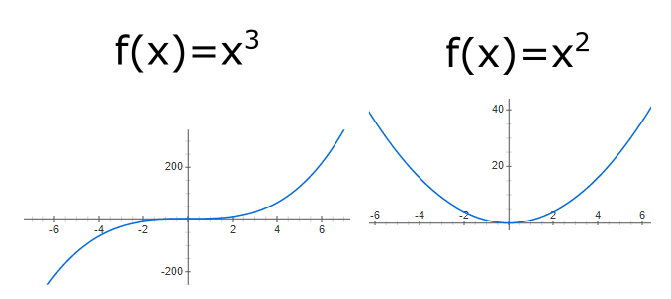
\includegraphics{C:/Users/gadia/Dropbox/Websites/blog/assets/img/2020/04/graphs.PNG}}

נעבור לתכונה השניה. פונקציה \L{$f:A\to B$} היא \textbf{על} \L{$B$}
אם לכל פלט אפשרי אכן קיים קלט שמחזיר אותו: כלומר, לכל \L{$b\in B$}
קיים \L{$a\in A$} כך ש-\L{$f\left(a\right)=b$}. למשל, אם לכל מילה
בשפה העברית \L{$f$} מתאימה את האות הראשונה שלה, אז זו פונקציה על
כי לכל אות בעברית קיימת מילה אחת לפחות שמתחילה באות הזו. לעומת זאת,
הפונקציה שמחזירה לכל אדם בישראל את מספר תעודת הזהות שלו איננה על כי
קיימים מספרים שאינם מספרי תעודת זהות. אבל רגע, הניסוח שלי קצת בעייתי
- לא אמרתי \textbf{על} מה הפונקציה הזו אמורה להיות. האם על קבוצת \textbf{כל}
המספרים הטבעיים? או אולי רק המספרים הטבעיים בני {\beginL 9\endL} ספרות
בדיוק? או אולי הקבוצה \textquotedblright כל המספרים הטבעיים שהם מספר
זהות של מישהו\textquotedblleft , מה שיגרום לפונקציה כן להיות על?

בואו נחזור אל שתי הפונקציות החביבות \L{$f\left(x\right)=x^{2}$} ו-\L{$f\left(x\right)=x^{3}$}
ונשאל את עצמנו - האם הן על? אם חושבים עליהן בתור פונקציות \L{$f:\mathbb{R}\to\mathbb{R}$},
אז \L{$f\left(x\right)=x^{2}$} בוודאי איננה על, כי \L{$-1$} אינו
הפלט של אף קלט. לעומת זאת \L{$f\left(x\right)=x^{3}$} היא כן על.
אפשר לראות את זה בתמונה: פונקציה היא על אם כל קו אופקי חותך אותה \textbf{לפחות
פעם אחת}.

על פניו, נראה שאם פונקציה אינה על קל \textquotedblright לתקן\textquotedblleft{}
את זה - פשוט נצמצם את הטווח שלה. למשל, עבור \L{$f\left(x\right)=x^{2}$}
אם נסתכל עליה בתור פונקציה \L{$f:\mathbb{R}\to[0,\infty)$} אז היא
בהחלט פונקציה על. אבל מה זה אומר, לצמצם את הטווח? זה אומר להחליף את
הפונקציה שלנו בפונקציה אחרת, שה\textquotedblleft כלל\textquotedblleft{}
שמגדיר אותה זהה. זה אומר שעברנו לסיטואציה אחרת, שהיא אולי מועילה יותר
בהקשר הנוכחי שלנו אבל לפעמים היא לא מועילה בכלל, ואני מקווה שזה יתברר
בקרוב מעצמו. עדיין, כדאי לדבר במפורש על ה\textquotedblleft תיקון\textquotedblleft{}
הזה: אם \L{$f:A\to B$} היא פונקציה כלשהי, \textbf{התמונה} של \L{$f$}
על \L{$A$} היא הקבוצה \L{$f\left(A\right)\triangleq\left\{ f\left(a\right)\ |\ a\in A\right\} $}
- זה אוסף האיברים ב-\L{$B$} שמתקבלים בעזרת \L{$f$}. עכשיו, אפשר
תמיד לומר ש-\L{$f:A\to f\left(A\right)$} היא על; ואפשר גם לומר שהתכונה
\textquotedblright להיות על\textquotedblleft{} היא פשוט הטענה \L{$B=f\left(A\right)$}.

אפשר באופן דומה גם \textquotedblright לתקן\textquotedblleft{} פונקציה
שאיננה חח\textquotedblleft ע על ידי צמצום של \textbf{התחום} שלה )כלומר,
של \L{$A$}(: בכל פעם שיש לנו זוג של איברים של \L{$A$} שמתמפים לאותו
פלט, פשוט להעיף אחד מהם מתוך \L{$A$}. לא הכי אלגנטי בעולם, אבל שימושי
בהקשרים מסויימים.

עכשיו, אחרי שראינו קצת את התכונות הללו, בואו ונראה מאיפה הן מגיעות.
ראשית, בואו נזכיר את שתי התכונות ש\textbf{מגדירות} מה זו פונקציה.
יחס \L{$f\subseteq A\times B$} הוא \textbf{פונקציה} אם מתקיים:
\begin{enumerate}
\item \textquotedblright קיום\textquotedblleft : לכל \L{$a\in A$} קיים
\L{$b\in B$} כך ש-\L{$\left(a,b\right)\in f$}.
\item \textquotedblright יחידות\textquotedblleft : אם \L{$\left(a,b_{1}\right)\in f$}
וגם \L{$\left(a,b_{2}\right)\in f$} עבור \L{$a\in A$} ו-\L{$b_{1},b_{2}\in B$}
אז \L{$b_{1}=b_{2}$}.
\end{enumerate}
עכשיו אני אנסח את תכונות ה\textquotedblleft על\textquotedblleft{} וה\textquotedblleft חד-חד-ערכית\textquotedblleft{}
באמצעות יחסים:
\begin{enumerate}
\item \textquotedblright על\textquotedblleft : לכל \L{$b\in B$} קיים \L{$a\in A$}
כך ש-\L{$\left(a,b\right)\in f$}
\item \textquotedblright חד-חד-ערכית\textquotedblleft : אם \L{$\left(a_{1},b\right)\in f$}
וגם \L{$\left(a_{2},b\right)\in f$} עבור \L{$a_{1},a_{2}\in A$}
ו-\L{$b\in B$} אז \L{$a_{1}=a_{2}$}.
\end{enumerate}
הדמיון בין תכונות הקיום/יחידות ותכונות העל/חח\textquotedblleft ע בולט
מאוד, כמובן. נראה שההגדרות כמעט זהות עד כדי החלפת תפקידים בין \L{$A$}
ו-\L{$B$}. ויש דרך לחדד את הדמיון עוד יותר אם \textbf{נהפוך} את \L{$f$}.
בואו נדבר על זה שניה.

\L{$f$} היא פונקציה, ומעבר למשמעות האינטואיטיבית של \textquotedblright משהו
שהופך קלט לפלט\textquotedblleft{} פונקציה היא קודם כל \textbf{יחס}
- אוסף של זוגות סדורים. אפשר פשוט לקחת כל זוג כזה ולהפוך את הסדר בין
האיברים שלו, והתוצאה נקראת \textbf{היחס ההפוך}. פורמלית, אם \L{$R\subseteq A\times B$}
הוא יחס כלשהו, מגדירים \L{$R^{-1}\triangleq\left\{ \left(b,a\right)\ |\ \left(a,b\right)\in R\right\} $}.
עכשיו עבור המקרה הפרטי של פונקציה \L{$f$} אפשר לעשות את אותו הדבר
בדיוק: להגדיר \L{$f^{-1}\triangleq\left\{ \left(b,a\right)\ |\ \left(a,b\right)\in f\right\} $},
ובסימון קצת יותר \textquotedblright פונקצייתי\textquotedblleft : \L{$f^{-1}\triangleq\left\{ \left(b,a\right)\ |\ f\left(a\right)=b\right\} $}.

מתי \L{$f^{-1}$} היא פונקציה? שימו לב לכך שהיחס \L{$f^{-1}$} \textbf{תמיד
קיים} אבל בהחלט \textbf{לא} מובטח שהוא יהיה פונקציה; פונקציה היא יחס
שמקיים שני תנאים ספציפיים, \textquotedblright קיום\textquotedblleft{}
ו\textquotedblleft יחידות\textquotedblleft , שפירושם עבור היחס \L{$f^{-1}\subseteq B\times A$}
הוא
\begin{enumerate}
\item \textquotedblright קיום\textquotedblleft : לכל \L{$b\in B$} קיים
\L{$a\in A$} כך ש-\L{$\left(b,a\right)\in f^{-1}$}.
\item \textquotedblright יחידות\textquotedblleft : אם \L{$\left(b,a_{1}\right)\in f^{-1}$}
וגם \L{$\left(b,a_{2}\right)\in f^{-1}$} עבור \L{$a_{1},a_{2}\in A$}
ו-\L{$b\in B$} אז \L{$a_{1}=a_{2}$}.
\end{enumerate}
עכשיו, במקום לכתוב \L{$\left(b,a\right)\in f^{-1}$} אני יכול לכתוב
\L{$\left(a,b\right)\in f$}: זו בדיוק ההגדרה של \L{$f^{-1}$}. וכעת
שתי השורות למעלה הופכות להיות:
\begin{enumerate}
\item \textquotedblright קיום\textquotedblleft : לכל \L{$b\in B$} קיים
\L{$a\in A$} כך ש-\L{$\left(a,b\right)\in f$}.
\item \textquotedblright יחידות\textquotedblleft : אם \L{$\left(a_{1},b\right)\in f$}
וגם \L{$\left(a_{2},b\right)\in f$} עבור \L{$a_{1},a_{2}\in A$}
ו-\L{$b\in B$} אז \L{$a_{1}=a_{2}$}.
\end{enumerate}
ואלו בדיוק, אבל בדיוק, התכונות של \textquotedblright על\textquotedblleft{}
ו\textquotedblleft חד-חד-ערכיות\textquotedblleft{} של \L{$f$}. אז
אפשר לסכם את מה שראינו במשפט אחד קצר וקולע: \L{$f$} היא חח\textquotedblleft ע
ועל אם ורק אם \L{$f^{-1}$} היא פונקציה. במקרה הזה נהוג להגיד ש-\L{$f$}
היא \textbf{הפיכה}. למה? כי אפשר לחשוב על \L{$f^{-1}$} בתור \textquotedblright אותה
הפונקציה כמו \L{$f$} רק בכיוון ההפוך\textquotedblleft . אם יש לנו
\L{$a\in A$} ואנחנו מפעילים את \L{$f$} על \L{$a$} ומקבלים \L{$f\left(a\right)=b$}
ואז מפעילים את \L{$f^{-1}$} על \L{$b$} אנחנו מקבלים \L{$f^{-1}\left(b\right)=a$},
כלומר \L{$f^{-1}\left(f\left(a\right)\right)=a$} - הפונקציה \L{$f^{-1}$}
\textquotedblright ביטלה\textquotedblleft{} את הפעולה של \L{$f$}.

פונקציות הפיכות הן כלי מרכזי בתורת הקבוצות - עליהן מתבססת ההגדרה שלנו
ל\textbf{שוויון עוצמות} של קבוצות, שבאה לתת גישה אפשרית אחת לשאלה
מתי שתי קבוצות )גם אינסופיות( הן מאותו גודל )ההגדרה פשוטה: \L{$A$}
שוות עוצמה ל-\L{$B$} אם קיימת \L{$f:A\to B$} הפיכה(. נדבר על זה
עוד בהמשך, אבל לפני כן אני ארצה לתת גישה מסודרת יותר לעניין ה\textquotedblleft מפעילים
את \L{$f$} על קלט ואז מפעילים משהו אחר על הפלט\textquotedblleft{}
- זה יוביל אותנו למושג ה\textbf{הרכבה} שעליו אדבר בפוסט הבא.
\end{document}
